%==============================================================================
\chapter{Detector}
\label{sec:det}
%==============================================================================

In this chapter, a detailed description of the proposed PINGU neutrino
telescope and its predecessor IceCube will be given. We will start with
introducing the concept of ice or water based neutrino telescopes based on the
detection of Cherenkov radiation with IceCube/DeepCore as example, followed by
a characterisation of its upcoming PINGU upgrade.
Thereafter we will discuss how physics events will be selected and
reconstructed in an analysis targeting the determination of the neutrino mass
hierarchy, and finally how conceptually new hardware might improve the results.

%==============================================================================
\section{IceCube/DeepCore}
\label{sec:ICDC}
%==============================================================================

\subsection{Location}
\label{sec:IClocation}

As already mentioned (Sec.~\ref{sec:NuDetection}), the natural choice for
observing the low natural fluxes of high energy neutrinos are water-based
Cherenkov detectors. Although the basic requirement---a sufficiently large
amount of water or ice---seems not very difficult to meet, there are additional
constraints that have to be addressed as well:

\begin{description}
 \item[Size:] Depending on the energy range one is interested in, the size of
  the detector has to be adjusted accordingly. Since the atmospheric flux
  decreases rapidly with increasing energy, one needs larger detectors to study
  higher fluxes. Roughly from the GeV scale upwards, the required dimensions are
  so big (several hundred metres) that artificial structures like the
  underground caverns of Kamiokande and Super-Kamiokande \cite{SuperKosc} are
  not feasible any more and one has to look for suitable natural locations.
 \item[Transparency:] Since the detection of neutrinos is based on recording
  Cherenkov radiation, i.\,e.\ photons in the optical and near UV regime,
  obviously the chosen medium has to be transparent for these photons. Here ice
  has an advantage over fluid water as it has very low absorption down to
  wavelengths of 300\,nm and below \cite{IceProps}, while the fluid starts to
  absorb significantly below 400\,nm \cite{WaterAbs}.
 \item[Purity:] Usually the experiments try to reconstruct the neutrino events
  as accurately as possible. Therefore it is desirable to record a large number
  of unscattered photons and hence a very clear environment\footnote{There might
  be, however, situations where scattering is desired, e.\,g.\ when only the
  neutrino energy is of interest, then strong scattering keeps the photons
  inside the detector for a longer time and hence increases the total number
  of detected photons, thereby improving the energy resolution}.
 \item[Shielding:] In high energy neutrino experiments, muons from atmospheric
  showers created by cosmic radiation (cf.\ Sec.~\ref{sec:AtmNus}) are a
  background process whose rate is several orders of magnitude higher than the
  neutrino signal. In order to suppress those muons, detectors have to be
  placed deep underground so that there is a shielding with several hundred
  meters thickness, comparable to the range of $\mathcal{O}
  (100\,\mathrm{GeV})$ muons.
\end{description}

\begin{figure}[htp]
 \centering
 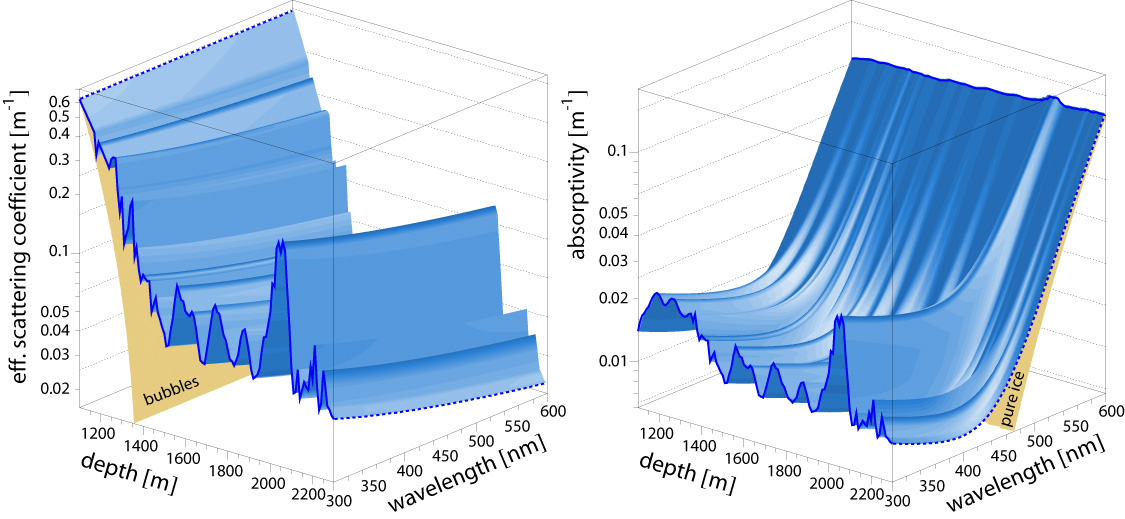
\includegraphics[width=\textwidth]{Icepaper_figure22_scatt-abs-length}
 \caption{Effective scattering and absorption of light in the polar ice. Plot 
  taken from \cite{IceProps}.}
 \label{fig:ice_scatt_abs}
\end{figure}

Choosing an environment optimising all these factors, the IceCube neutrino 
observatory has been constructed in the deep glacial ice at the geographical 
South Pole in Antarctica. The Antarctic glacier with its thickness of $\approx 
2500$\,m is a pristine environment of substantial size. In contrast to natural 
resources like lakes or the deep sea, it inherently provides a solid holding 
structure for the instrumentation, is free of lifeforms that might disturb or 
even destroy the detector, and has a much lower content of radioactive $^{40}$K 
than sea water. Especially at depths more than $\approx 2000$\,m below the 
surface, age and high pressure have facilitated the hydratisation of enclosed 
air bubbles, leaving an extremely clear ice with scattering and absorption 
lengths of several tens of metres even in the UV range, see 
Fig.~\ref{fig:ice_scatt_abs}. Instrumenting only the deepest ice below 1500\,m 
guarantees a sufficient shielding of atmospheric muons. 

The nearby Amundsen-Scott South Pole Station operated by the United States 
Antarctic Program provides the infrastructure needed for such a large scale 
experiment. This incorporates the supply of electrical power for the detector 
itself and the computing farm processing the raw data, satellite communications 
for transmitting science data, general technical support as well as 
accommodations for the visiting scientists.

\subsection{Detector Geometry}
\label{sec:ICgeometry}

A total of 86 strings, each instrumented with 60 Digital Optical Modules (DOMs, 
see Sec.~\ref{sec:ICDOM}), have been installed during IceCube's deployment phase 
from 2005 until December 18, 2010. A hot water drill was used to melt holes of 
60\,cm diameter into the ice, reaching down to 2450\,m, shortly above the 
underlying bedrock. Then the strings were lowered into the holes still filled 
with water which then refroze and firmly encloses the strings.

Eighty of those strings form the hexagonal main array with an inter-string 
distance of 125\,m, while the remaining six are placed at additional positions 
near the centre of the array, forming a dense sub-array with a string spacing 
of only 72\,m, lowering the threshold energy for neutrino detection from 
$\approx 100$\,GeV to $\approx 20$\,GeV. A top view of the string layout is 
shown in Fig.\ref{fig:string_layout}.

\begin{figure}[htp]
 \centering
%  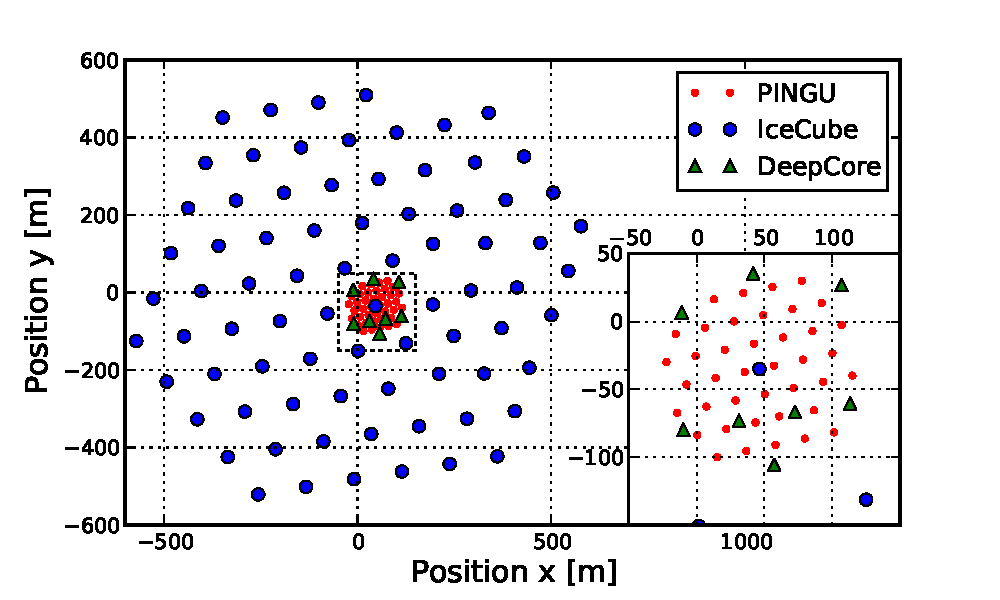
\includegraphics[width=\textwidth]{ic_dc_pingu_strings}
 \caption{Top view of the IceCube string layout, including the DeepCore and 
planned PINGU (geometry V36) sub-arrays.}
 \label{fig:string_layout}
\end{figure}


\cite{I3Design,DCDesign}


\subsection{Digital Optical Modules}
\label{sec:ICDOM}


%==============================================================================
\section{PINGU}
\label{sec:PINGU}
%==============================================================================


%==============================================================================
\section{Event Selection}
\label{sec:EvtSel}
%==============================================================================


%==============================================================================
\section{Event Reconstruction}
\label{sec:EvtReco}
% TODO: maybe move this section to the end of the chapter?
%==============================================================================


%==============================================================================
\section{Next-Generation Optical Modules}
\label{sec:EvtReco}
%==============================================================================

\subsection{Wavelength-shifting Optical Module (WOM)}


\subsection{Multi-PMT Optical Module (mDOM)}